\documentclass{article}
\usepackage[utf8]{inputenc}
\usepackage[margin=7mm]{geometry}
\usepackage{pgf}
\usepackage{pgfcore}
\usepackage{pgfbaseimage}
\usepackage{pgfbaselayers}
\usepackage{pgfbasepatterns}
\usepackage{pgfbaseplot}
\usepackage{pgfbaseshapes}
\usepackage{pgfbasesnakes}
\pagestyle{empty}
\usepackage{tikz}
\usepackage{url}

%\usepackage[active,pdftex,tightpage]{preview}
%\PreviewEnvironment[{[]}]{tikzpicture}
%\parskip=0.5\baselineskip
\newcommand{\li}{\linewidth}
\newcommand{\hi}{\heighwidth}
\newcommand{\marge}{0.03\li}
\newcommand{\margeb}{0.52\li}
\newcommand{\ra}{4.5} 
\newcommand{\rf}{1.3}
% commande pour choisir la taille de police avec interligne automatique
\newcommand{\autofontsize}[1]{\fontsize{#1}{\dimexpr #1*12/10}}

%\colorlet{colmotif}{black!50}
\definecolor{violetmmi}{RGB}{144,64,152}
\definecolor{vertmmi}{RGB}{158,204,59}
\colorlet{colmotif}{violetmmi}

\tikzstyle{pli}=[help lines]
\tikzstyle{bord}=[line width=1pt]
\tikzstyle{noeud}=[minimum size=0, inner sep =0]
\tikzstyle{motif}=[fill,colmotif]

%dessine le recto : premier argument = position, deuxieme argument = rotation
\newcommand{\recto}[2]{
  \begin{scope}[shift={#1}]
  \begin{scope}[rotate=#2]
    \begin{scope}[shift={(-60:\ra)}]
  \foreach \I in {0,...,5}
{\node[noeud](A\I) at (\I*\ra,0) {};
\draw (A\I)++(120:\ra) node[noeud](B\I) {};
\draw[pli] (A\I) -- (B\I);
}

\foreach \I in {0,1,...,4}
\draw[pli] (A\I)--++(60:\ra);
\path[draw,bord,join=miter] (0,0) -- (5*\ra,0) -- ++(120:\ra)-- (120:\ra)-- cycle;

\draw (90:\ra/2) node[rotate=#2] {C};
\draw (4.5*\ra,0)++(90:\ra/3) node[rotate=#2] {C};

%motifs 1

 \draw[motif] (0,0) -- +(\rf,0) --+(30:\rf*1.6)-- +(60:\rf) -- cycle;
\draw[motif] (3*\ra,0)-- +(\rf,0) --+(30:\rf*1.6)-- +(60:\rf) --+(90:\rf*1.6)-- +(120:\rf) -- cycle;


%motifs 2

\draw[motif] (2*\ra,0) -- ++(\rf,0) -- ++(120:\rf) -- ++(-\rf,0) -- cycle;

%motifs 3

\draw[colmotif,line width=5pt] (\ra,0)++(\ra/3,0) arc (0:120:\ra/3);
\draw[colmotif,line width=5pt] (4*\ra,0)++(60:\ra/3) arc (60:120:\ra/3);

\path[draw,bord,join=miter] (0,0) -- (5*\ra,0) -- ++(120:\ra)-- (120:\ra)-- cycle;
\end{scope}
    \end{scope}
    \end{scope}

  }

\newcommand\verso[2]{
  \begin{scope}[shift={#1}]
\begin{scope}[rotate=#2]
  \foreach \I in {0,...,5}
{\node[noeud](A\I) at (\I*\ra,0) {};
\draw (A\I)++(60:\ra) node[noeud](B\I) {};
\draw[pli] (A\I) -- (B\I);
}

\foreach \I in {1,...,4,5}
\draw[pli] (A\I)--++(120:\ra);

%motifs 1

\draw[fill,colmotif] (5*\ra,0) -- +(60:\rf) --+(90:\rf*1.6)-- +(120:\rf) -- cycle;
\draw[fill,colmotif] (2*\ra,0) -- +(\rf,0) --+(30:\rf*1.6)-- +(60:\rf) --+(90:\rf*1.6)-- +(120:\rf) -- cycle;


%motifs 2
%\draw[fill,colmotif] (\ra,0)++(60:\ra) -- ++(-\rf,0) -- ++(-60:\rf) -- ++(\rf,0) -- cycle;
%\draw[fill,colmotif] (4*\ra,0)++(60:\ra) -- ++(-\rf,0) -- ++(-60:\rf) -- ++(\rf,0) -- cycle;


\draw[motif] (\ra,0) -- ++(\rf,0) -- ++(120:\rf) -- ++(-\rf,0) -- cycle;
\draw[motif] (4*\ra,0) -- ++(\rf,0) -- ++(120:\rf) -- ++(-\rf,0) -- cycle;


%motifs 3

\draw[line width=5pt,colmotif] (0,0)++(\ra/3,0) arc (0:60:\ra/3);
\draw[line width=5pt,colmotif] (3*\ra,0)++(0:\ra/3) arc (0:120:\ra/3);

\path[draw,bord,join=miter] (0,0) -- (5*\ra,0) -- ++(60:\ra)-- (60:\ra)-- cycle;
\end{scope}
\end{scope}
}

 \begin{document}
 \centering
 \scalebox{1} {
 \begin{tikzpicture}
\clip (0.5,0.5) rectangle (20,27);
\recto{(1.5,1)}{90}

\node at (17,2) {(logo)};%\includegraphics[width=5cm]{logo-MMI.png}};

\node at (12,26) {\Huge \bf \color{violetmmi} Construire son {\color{vertmmi}flexa}gone};

\node at (13,23) {
  \parbox{12cm}{
    {\bf \color{violetmmi} \'Etape 1 :} Découper le patron et plier suivant les pointillés.

    \vspace{-0.5cm}
    \begin{center}
      \scalebox{0.3}{\begin{tikzpicture}[anchor=center]
          \recto{(0,0)}{0}
          \draw[line width=4pt, loosely dotted] (3*\ra,0)++(-120:1.5*\ra) -- ++(60:2*\ra);

          \path[draw, line width=2pt,->] (3*\ra,0)++(-120:1.5*\ra)++(120:0.2*\ra) arc (150:300:\ra/4);

      \end{tikzpicture}}
       \end{center}
}}
;

\node at (13,19) {
  \parbox{12cm}{
    {\bf \color{violetmmi} \'Etape 2 :} Plier suivant les pointillés.

 %   \vspace{-0.5cm}
    \begin{center}
      \scalebox{0.3}{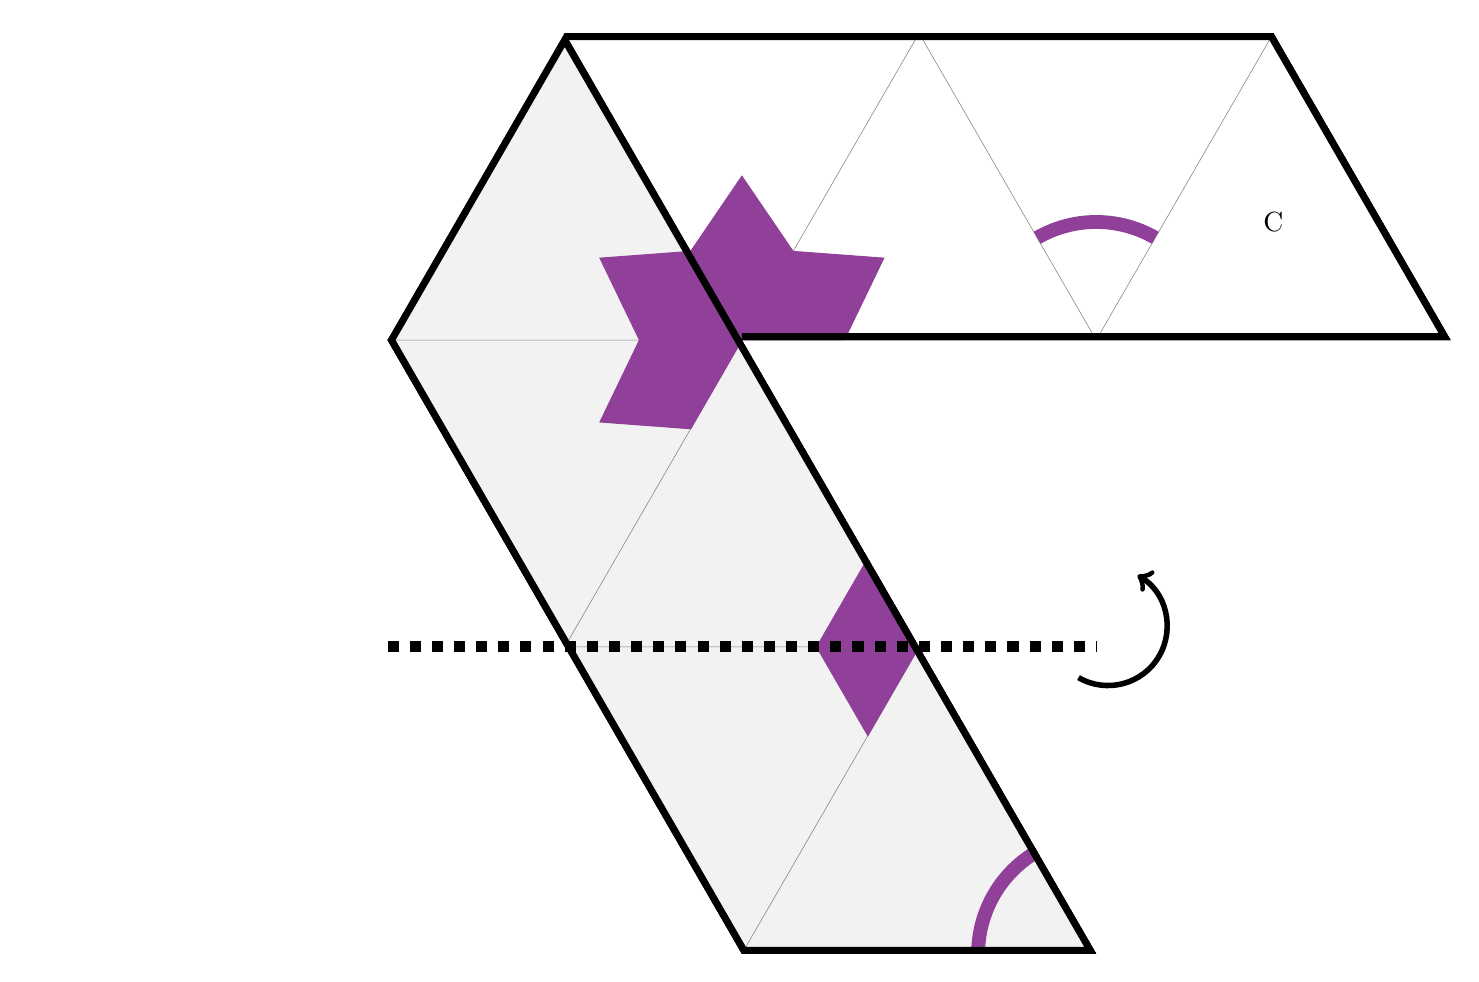
\begin{tikzpicture}
 \begin{scope}
      \clip (3*\ra,0) -- (5*\ra,0)-- ++(-60:\ra) --++(-2*\ra,0) --cycle;
            \recto{(0,0)}{0}
 \draw[line width=5pt] (3*\ra,0) -- (5*\ra,0)-- ++(-60:\ra) --++(-2*\ra,0) ;
     
 \end{scope}
     
          \begin{scope}[shift={(-60:3*\ra)}]
           
           
            \clip (3*\ra,0) --  ++(120:3*\ra) -- ++(-120:\ra) --++(-60:2*\ra)--cycle;
 \draw[fill=black!5]  (3*\ra,0) --  ++(120:3*\ra) -- ++(-120:\ra) --++(-60:2*\ra)--cycle;
            
            \verso{(3*\ra,0)}{120}
  \draw[line width =5pt]  (3*\ra,0) --  ++(120:3*\ra) -- ++(-120:\ra) --++(-60:2*\ra)--cycle;

          \end{scope}

             \draw[line width=4pt, loosely dotted] (1.5*\ra,0)++(-60:2*\ra) -- ++(2*\ra,0);

          \path[draw, line width=2pt,->] (3.5*\ra,0)++(-60:2*\ra)++(-120:0.1*\ra) arc (-120:60:\ra/6);

          \end{tikzpicture}}
       \end{center}
}}
;


\node at (13,13.5) {
  \parbox{12cm}{
    {\bf \color{violetmmi} \'Etape 3 :} Plier en arrière suivant les pointillés et glisser le dernier triangle sur le pliage de fa\c{c}on à superposer les deux 'C'.

 %   \vspace{-0.5cm}
    \begin{center}
      \scalebox{0.3}{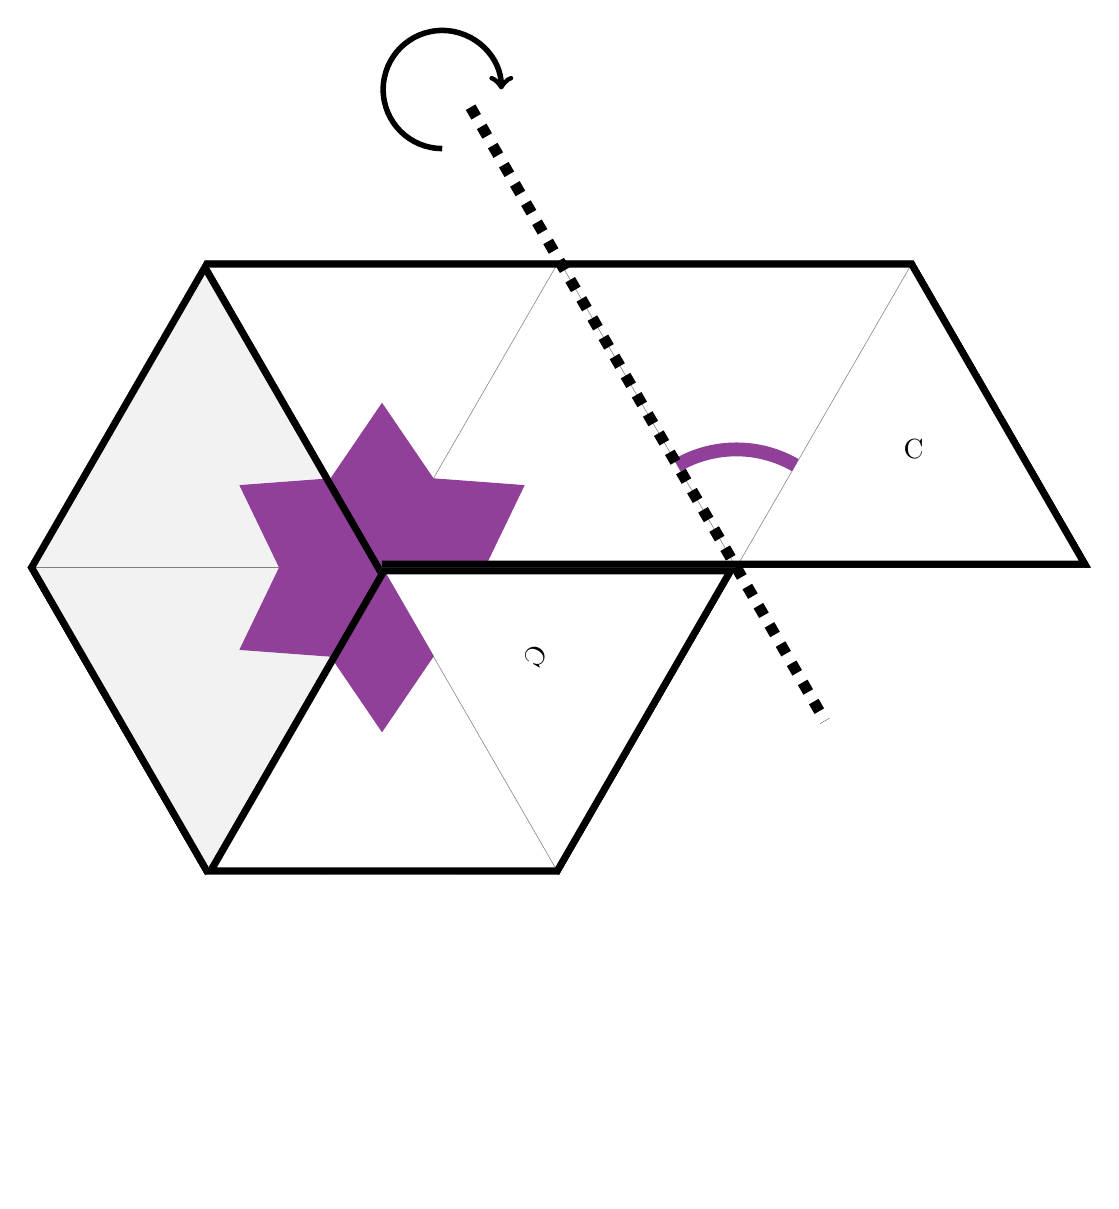
\begin{tikzpicture}
 \begin{scope}
      \clip (3*\ra,0) -- (5*\ra,0)-- ++(-60:\ra) --++(-2*\ra,0) --cycle;
            \recto{(0,0)}{0}
 \draw[line width=5pt] (3*\ra,0) -- (5*\ra,0)-- ++(-60:\ra) --++(-2*\ra,0) ;
     
 \end{scope}
     
          \begin{scope}[shift={(-60:3*\ra)}]
           
           
            \clip (2*\ra,0)++(60:\ra) --  ++(120:2*\ra) -- ++(-120:\ra) --++(-60:\ra)--cycle;

        \draw[fill=black!5] (2*\ra,0)++(60:\ra) --  ++(120:2*\ra) -- ++(-120:\ra) --++(-60:\ra)--cycle;
          
            \verso{(3*\ra,0)}{120}
            \draw[line width =5pt] (2*\ra,0)++(60:\ra) --  ++(120:2*\ra) -- ++(-120:\ra) --++(-60:\ra)--cycle;
          \end{scope}

          \begin{scope}[shift={(-120:\ra)}]
      \clip (4*\ra,0) -- (5*\ra,0)-- ++(-120:\ra) --++(-\ra,0) --cycle;
 \path[fill=white] (4*\ra,0) -- (5*\ra,0)-- ++(-120:\ra) --++(-\ra,0) --cycle;
     
      \recto{(5*\ra,0)}{-120}
   \draw[line width=5pt](4*\ra,0) -- (5*\ra,0)-- ++(-120:\ra) --++(-\ra,0) --cycle;
        
 \end{scope}

          \draw[line width=4pt, loosely dotted] (4*\ra,0)++(120:0.5*\ra) -- ++(-60:2*\ra);

          \path[draw, line width=2pt,<-] (4*\ra,0)++(120:0.5*\ra)++(30:0.1*\ra) arc (0:270:\ra/6);

          \end{tikzpicture}}
       \end{center}
}}
;

\node at (13,9.5) {
  \parbox{12cm}{
    {\bf \color{violetmmi} \'Etape 4 :} Coller les deux 'C' entre eux. 

 %   \vspace{-0.5cm}
    \begin{center}
      \scalebox{0.3}{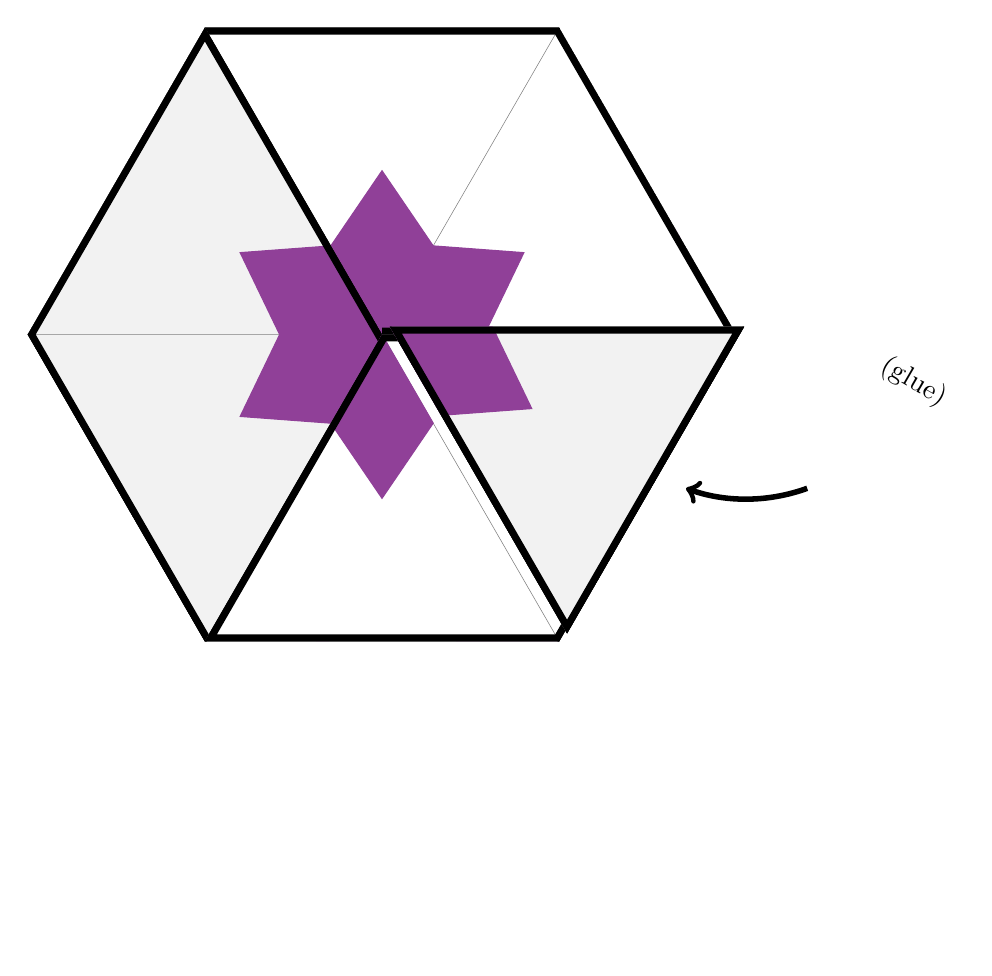
\begin{tikzpicture}
 \begin{scope}
      \clip (3*\ra,0) -- (4*\ra,0)-- ++(-60:\ra) --++(-\ra,0) --cycle;
            \recto{(0,0)}{0}
 \draw[line width=5pt] (3*\ra,0) -- (4*\ra,0)-- ++(-60:\ra) --++(-\ra,0) ;
     
 \end{scope}
     
          \begin{scope}[shift={(-60:3*\ra)}]
           
           
            \clip (2*\ra,0)++(60:\ra) --  ++(120:2*\ra) -- ++(-120:\ra) --++(-60:\ra)--cycle;

        \draw[fill=black!5] (2*\ra,0)++(60:\ra) --  ++(120:2*\ra) -- ++(-120:\ra) --++(-60:\ra)--cycle;
          
            \verso{(3*\ra,0)}{120}
            \draw[line width =5pt] (2*\ra,0)++(60:\ra) --  ++(120:2*\ra) -- ++(-120:\ra) --++(-60:\ra)--cycle;
          \end{scope}

          \begin{scope}[shift={(-120:\ra)}]
      \clip (4*\ra,0) -- (5*\ra,0)-- ++(-120:\ra) --++(-\ra,0) --cycle;
 \path[fill=white] (4*\ra,0) -- (5*\ra,0)-- ++(-120:\ra) --++(-\ra,0) --cycle;
     
      \recto{(5*\ra,0)}{-120}
   \draw[line width=5pt](4*\ra,0) -- (5*\ra,0)-- ++(-120:\ra) --++(-\ra,0) --cycle;
        
 \end{scope}

               \begin{scope}[shift={(60:4*\ra)}]
            %     \draw[line width =5pt, red]  (0,0)++(-60:5*\ra) circle (0.2cm);
  \clip (-60:5*\ra)++(0.1,0.1) --  ++(-\ra,0) -- ++(-60:\ra) --cycle;
      
        \draw[fill=black!5] (0.1,0.1)++(-60:5*\ra) --  ++(-\ra,0) -- ++(-60:\ra) --cycle;
          
            \verso{(4*\ra+0.1,0.1)}{-120}
   \draw[line width=5pt] (0.1,0.1)++(-60:5*\ra) --  ++(-\ra,0) -- ++(-60:\ra) --cycle;

               \end{scope}
               
               \draw (5*\ra,-\ra) node[rotate=-30] {(glue)};%\includegraphics[width=3cm]{glue.jpg}};
               
          \path[draw, line width=2pt,->] (4.7*\ra,-1.3*\ra) arc (-70:-110:\ra/2);

      \end{tikzpicture}}

       \end{center}
}}
;
\node at (13,5) {
  \parbox{12cm}{
    {\bf \color{violetmmi} \'Etape 5 :} Marquer les plis intérieurs en pliant et dépliant suivant les pointillés. Votre flexagone est prêt, pour le faire fonctionner, regarder au dos !

 %   \vspace{-0.5cm}
    \begin{center}
      \scalebox{0.3}{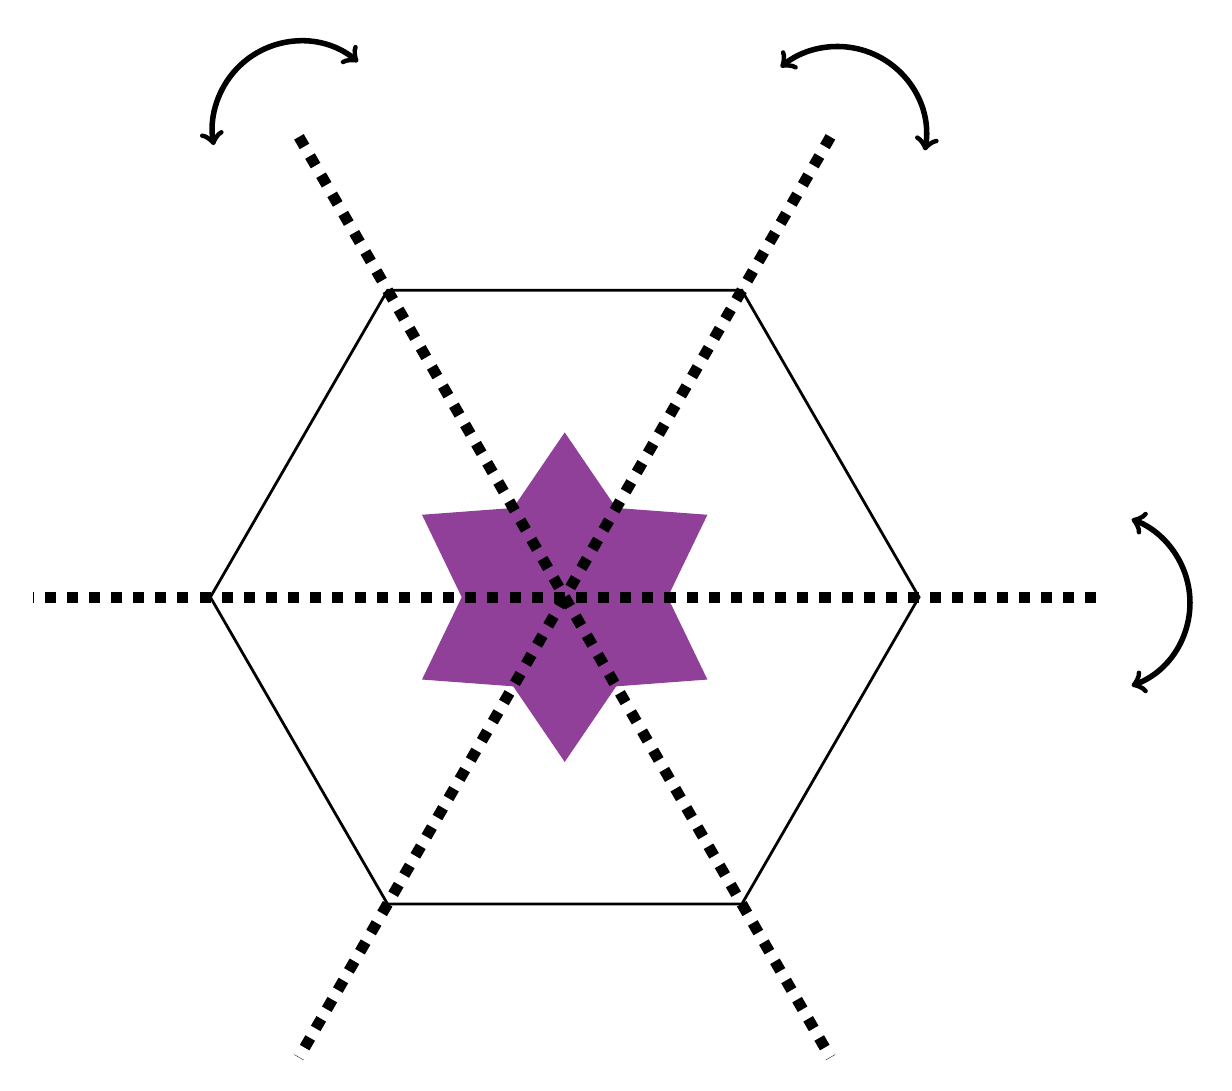
\begin{tikzpicture}

\draw[bord] (0:\ra) -- (60:\ra) -- (120:\ra) -- (180:\ra) -- (240:\ra) -- (300:\ra) -- cycle;       

\foreach \a in {0,60,...,300}
\draw[motif] (\a:\rf) --(\a+30:\rf*1.6)--(\a+60:\rf) --(0,0)-- cycle;

\draw[line width=4pt, loosely dotted] (0:1.5*\ra) -- (180:1.5*\ra);
\draw[line width=4pt, loosely dotted] (60:1.5*\ra) -- (240:1.5*\ra);
\draw[line width=4pt, loosely dotted] (120:1.5*\ra) -- (300:1.5*\ra);

               
\foreach \a in {0,60,120}
\path[draw, line width=2pt,<->] (\a:1.6*\ra)++(\a-90:\ra/4) arc (-70+\a:70+\a:\ra/4);

      \end{tikzpicture}}

       \end{center}
}}
;

 \end{tikzpicture}
 }
\newpage
\scalebox{1}{
\begin{tikzpicture}
  \clip (0.5,0.5) rectangle (20,27);
  \verso{(19,1)}{90}

  \node at (9,26) {\Huge \bf \color{violetmmi} Utiliser son {\color{vertmmi}flexa}gone};
\node at (7,23) {
  \parbox{12cm}{
    {\bf \color{violetmmi} \'Etape 1 :} Plier un pli sur deux en montagne, aux endroits où il y a une ouverture du papier. Une fois plié, cela doit ressembler aux images de droite.
    
 %   \vspace{-0.5cm}
  \begin{center}
     \scalebox{0.3}{\begin{tikzpicture}
\draw[bord] (0:\ra) -- (60:\ra) -- (120:\ra) -- (180:\ra) -- (240:\ra) -- (300:\ra) -- cycle;       

\foreach \a in {0,60,...,300}
\draw[motif] (\a:\rf) --(\a+30:\rf*1.6)--(\a+60:\rf) --(0,0)-- cycle;


\draw[line width=5pt,loosely dotted] (0,0) -- (0:\ra);
\draw[line width=5pt,loosely dotted] (0,0) -- (120:\ra);
\draw[line width=5pt,loosely dotted] (0,0) -- (240:\ra);
\draw[line width=1pt] (0,0) -- (60:\ra);
\draw[line width=1pt] (0,0) -- (180:\ra);
\draw[line width=1pt] (0,0) -- (300:\ra);


\foreach \a in {60,180,300}
\path[draw, line width=2pt,->] (\a:1.3*\ra) -- (\a:1.1*\ra);

\foreach \a in {0,120,240}
\path[draw, line width=2pt,<->] (\a:1.3*\ra)++(\a+140:\ra/4) arc (140+\a:220+\a:\ra/4);

\path[line width=5pt, ->, draw] (1.5*\ra,0) -> (2*\ra,0);

\begin{scope}[shift={(3*\ra,0)}]


  \draw[bord] (0:\ra)--(60:0.2*\ra)--(120:\ra) -- (180:0.2*\ra)--(240:\ra)--(300:0.2*\ra)--cycle;
\foreach \a in {0,120,240}
  {\draw[motif] (\a:0.9*\rf)--(\a+20:1*\rf)--(\a+60:0.3*\rf) -- (0,0)--cycle;
  \draw[motif] (\a:0.9*\rf)--(\a-20:1*\rf)--(\a-60:0.3*\rf) -- (0,0)--cycle;
  }
  \foreach \a in {60,180,300}
  \path[draw] (\a:0.2*\ra) -- (0,0);

   \draw[line width=4pt] (0,0)--(0:0.95*\ra);
  \draw[line width=4pt] (0,0)--(120:0.95*\ra);
  \draw[line width=4pt] (0,0)--(240:0.95*\ra);

  \node at (0,-1.2*\ra) {\Huge Vu du dessus};
\end{scope}

\begin{scope}[shift={(5.5*\ra,0.5*\ra)}]

  \draw[line width=4pt] (0,0) -- (-30:\ra) -- coordinate[pos=0.8](d) (0,-0.1*\ra)coordinate (d3) --
  coordinate[pos=0.2](d2) (-135:\ra)--coordinate[pos=0.8](d4) (-0.1*\ra,-0.1*\ra) coordinate(d6) --coordinate[pos=0.3](d5) (-160:\ra)--cycle;
  
  \draw[bord] (-160:\ra)--(-135:0.8*\ra) (-135:\ra) -- (-90:\ra) -- (-30:\ra);

  \draw (0,-0.1*\ra) -- (-90:\ra);
  
\draw[motif] (0,-0.1*\ra)--(d)--(-65:1.5*\rf) -- (-90:\rf)--(-110:1.6*\rf)--(d2) -- (d3);
\draw[motif] (d4)--(d5)--(d6)--cycle;

\draw[line width=4pt] (0,0) -- (-30:\ra) -- coordinate[pos=0.8](d) (0,-0.1*\ra)coordinate (d3) --
  coordinate[pos=0.2](d2) (-135:\ra)-- (-0.1*\ra,-0.1*\ra) -- (-160:\ra)--cycle;
 
  \node at (0,-1.7*\ra) {\Huge Vu de c\^ot\'e};
  \end{scope}
      \end{tikzpicture}}

       \end{center}
}}
;

\node at (7,18) {
  \parbox{12cm}{
    {\bf \color{violetmmi} \'Etape 2 :} Ouvrir le flexagone par le centre. Vous devez obtenir l'image de droite. Si vous n'arrivez pas à ouvrir, inverser tous les plis à l'étape précédente.
    
 %   \vspace{-0.5cm}
    \begin{center}
      \scalebox{0.3}{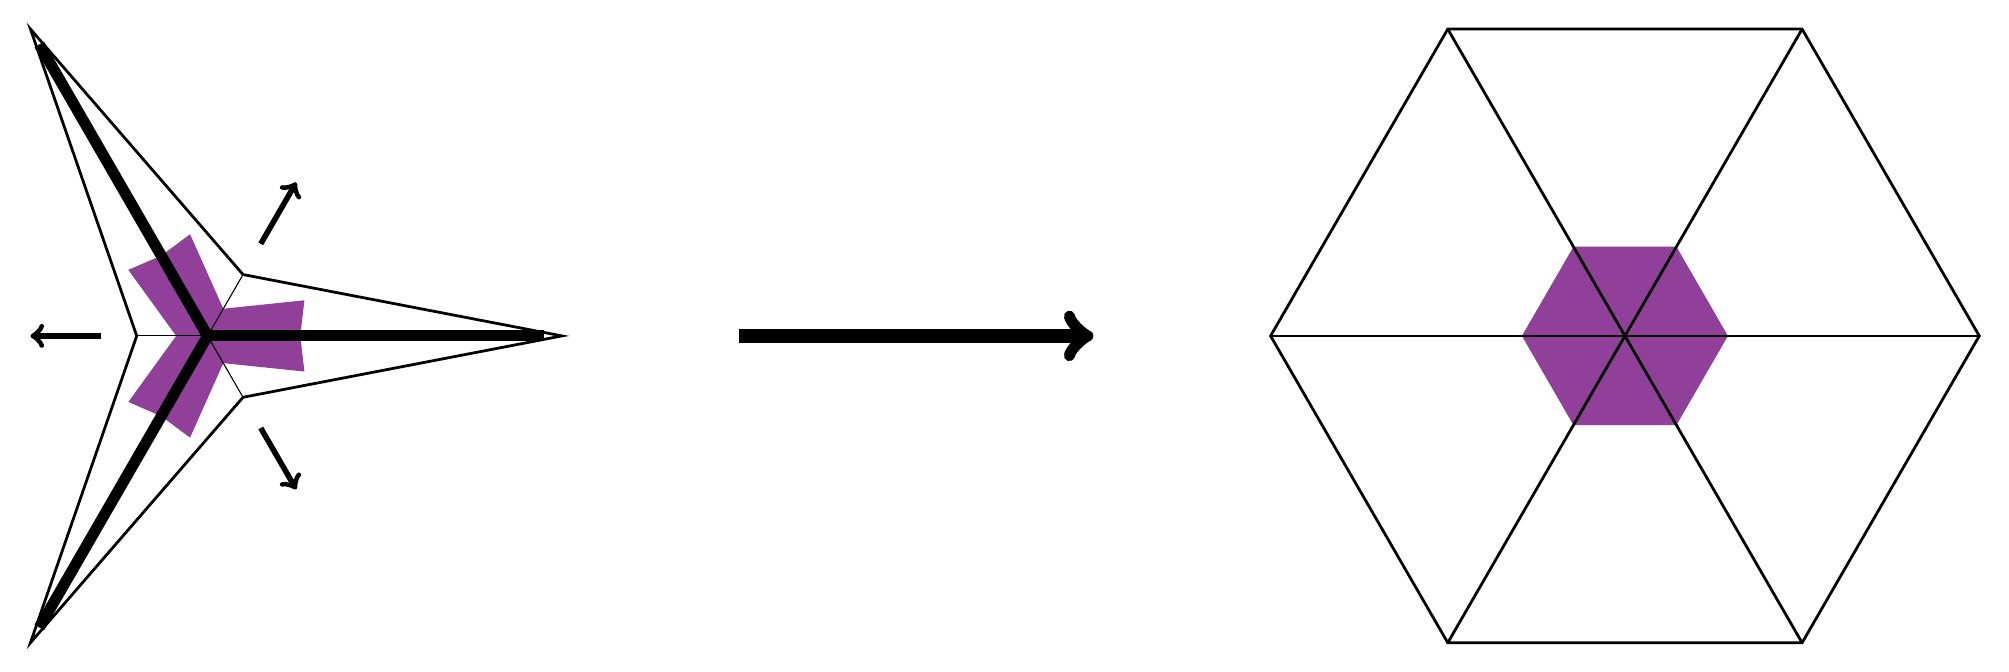
\begin{tikzpicture}

          \begin{scope}[shift={(0,0)}]

  \draw[bord] (0:\ra)--(60:0.2*\ra)--(120:\ra) -- (180:0.2*\ra)--(240:\ra)--(300:0.2*\ra)--cycle;
\foreach \a in {0,120,240}
  {\draw[motif] (\a:0.9*\rf)--(\a+20:1*\rf)--(\a+60:0.3*\rf) -- (0,0)--cycle;
  \draw[motif] (\a:0.9*\rf)--(\a-20:1*\rf)--(\a-60:0.3*\rf) -- (0,0)--cycle;
  }
  \foreach \a in {60,180,300}
  \path[draw] (\a:0.2*\ra) -- (0,0);

   \draw[line width=4pt] (0,0)--(0:0.95*\ra);
  \draw[line width=4pt] (0,0)--(120:0.95*\ra);
  \draw[line width=4pt] (0,0)--(240:0.95*\ra);

  \foreach \a in {60,180,300}
  \path[draw,->,line width=2pt] (\a:0.3*\ra) -> (\a:0.5*\ra);
  
  \end{scope}

          \path[line width=5pt, ->, draw] (1.5*\ra,0) -> (2.5*\ra,0);

          \begin{scope}[shift={(4*\ra,0)}]
          
\draw[bord] (0:\ra) -- (60:\ra) -- (120:\ra) -- (180:\ra) -- (240:\ra) -- (300:\ra) -- cycle;       

\foreach \a in {0,60,...,300}
\draw[motif] (\a:\rf) -- (\a+60:\rf)--(0,0)-- cycle;


\draw[line width=1pt] (0,0) -- (0:\ra);
\draw[line width=1pt] (0,0) -- (120:\ra);
\draw[line width=1pt] (0,0) -- (240:\ra);
\draw[line width=1pt] (0,0) -- (60:\ra);
\draw[line width=1pt] (0,0) -- (180:\ra);
\draw[line width=1pt] (0,0) -- (300:\ra);

\end{scope}


      \end{tikzpicture}}

       \end{center}
}}
;

 \node at (7,10) {
   \parbox{12cm}{
     {\bf \color{violetmmi} \'Etape 3 :} Recommencez les étapes 1 et 2 pour trouver le troisième motif. Avec cette opération et celle consistant à retourner le flexagone, vous devez pouvoir obtenir toutes les faces qui suivent :

\begin{center}
\scalebox{0.2}{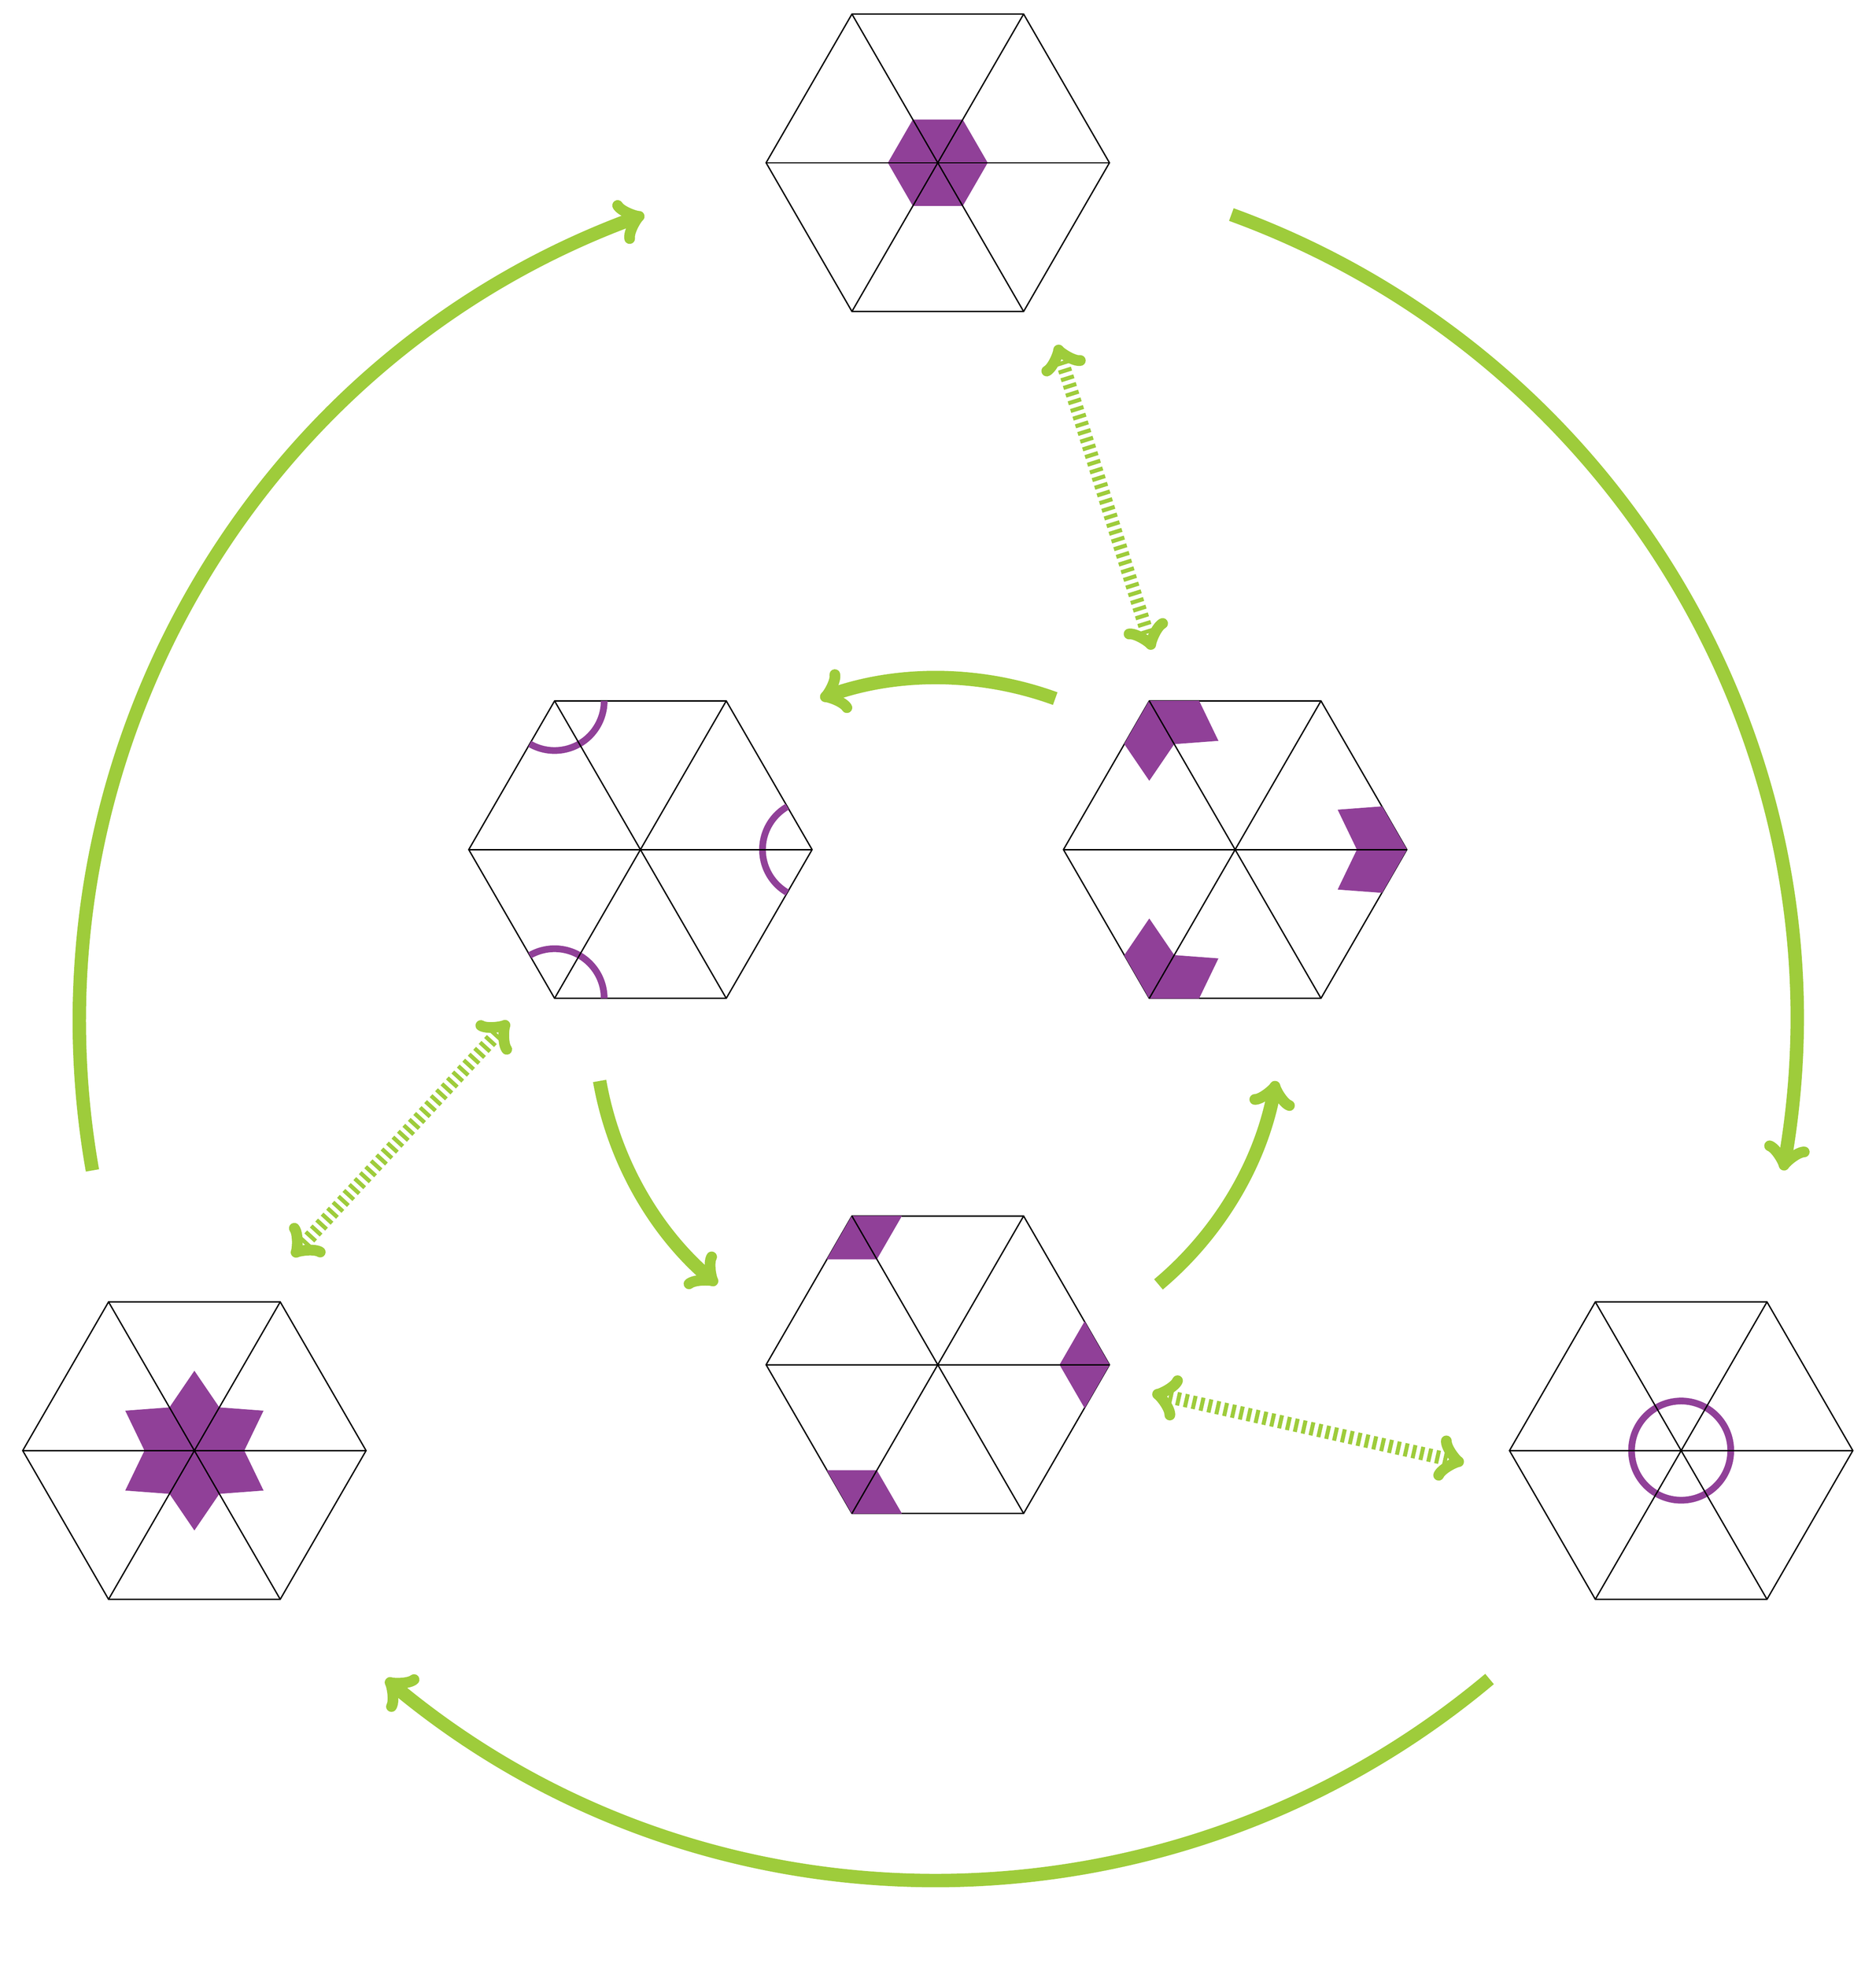
\begin{tikzpicture}

\begin{scope}[shift={(30:2*\ra)}]
          
\draw[bord] (0:\ra) -- (60:\ra) -- (120:\ra) -- (180:\ra) -- (240:\ra) -- (300:\ra) -- cycle;       

\foreach \a in {0,120,240}
\draw[motif] (\a:\ra)--+(-120+\a:\rf) -- +(\a-150:1.6*\rf)--+(\a-180:\rf)--+(\a+150:1.6*\rf)--+(\a+120:\rf)-- cycle;


\draw[line width=1pt] (0,0) -- (0:\ra);
\draw[line width=1pt] (0,0) -- (120:\ra);
\draw[line width=1pt] (0,0) -- (240:\ra);
\draw[line width=1pt] (0,0) -- (60:\ra);
\draw[line width=1pt] (0,0) -- (180:\ra);
\draw[line width=1pt] (0,0) -- (300:\ra);

\end{scope}

\begin{scope}[shift={(90:5*\ra)}]
          
\draw[bord] (0:\ra) -- (60:\ra) -- (120:\ra) -- (180:\ra) -- (240:\ra) -- (300:\ra) -- cycle;       

\foreach \a in {0,60,...,300}
\draw[motif] (\a:\rf) -- (\a+60:\rf)--(0,0)-- cycle;


\draw[line width=1pt] (0,0) -- (0:\ra);
\draw[line width=1pt] (0,0) -- (120:\ra);
\draw[line width=1pt] (0,0) -- (240:\ra);
\draw[line width=1pt] (0,0) -- (60:\ra);
\draw[line width=1pt] (0,0) -- (180:\ra);
\draw[line width=1pt] (0,0) -- (300:\ra);

\end{scope}

\begin{scope}[shift={(150:2*\ra)}]
          
\draw[bord] (0:\ra) -- (60:\ra) -- (120:\ra) -- (180:\ra) -- (240:\ra) -- (300:\ra) -- cycle;       

\foreach \a in {0,120,240}
\draw[colmotif,line width=5pt] (\a:\ra)++(\a+120:\rf) arc (\a+120:\a+240:\rf);


\draw[line width=1pt] (0,0) -- (0:\ra);
\draw[line width=1pt] (0,0) -- (120:\ra);
\draw[line width=1pt] (0,0) -- (240:\ra);
\draw[line width=1pt] (0,0) -- (60:\ra);
\draw[line width=1pt] (0,0) -- (180:\ra);
\draw[line width=1pt] (0,0) -- (300:\ra);

\end{scope}

\begin{scope}[shift={(-90:2*\ra)}]
          
\draw[bord] (0:\ra) -- (60:\ra) -- (120:\ra) -- (180:\ra) -- (240:\ra) -- (300:\ra) -- cycle;       

\foreach \a in {0,120,240}
\draw[motif] (\a:\ra) -- +(\a+120:\rf)--+(\a+180:\rf)--+(\a+240:\rf)-- cycle;


\draw[line width=1pt] (0,0) -- (0:\ra);
\draw[line width=1pt] (0,0) -- (120:\ra);
\draw[line width=1pt] (0,0) -- (240:\ra);
\draw[line width=1pt] (0,0) -- (60:\ra);
\draw[line width=1pt] (0,0) -- (180:\ra);
\draw[line width=1pt] (0,0) -- (300:\ra);

\end{scope}

\begin{scope}[shift={(330:5*\ra)}]
          
\draw[bord] (0:\ra) -- (60:\ra) -- (120:\ra) -- (180:\ra) -- (240:\ra) -- (300:\ra) -- cycle;       

\draw[colmotif,line width=5pt] (0,0) circle (\rf cm); 

\draw[line width=1pt] (0,0) -- (0:\ra);
\draw[line width=1pt] (0,0) -- (120:\ra);
\draw[line width=1pt] (0,0) -- (240:\ra);
\draw[line width=1pt] (0,0) -- (60:\ra);
\draw[line width=1pt] (0,0) -- (180:\ra);
\draw[line width=1pt] (0,0) -- (300:\ra);

\end{scope}

\begin{scope}[shift={(210:5*\ra)}]
          
\draw[bord] (0:\ra) -- (60:\ra) -- (120:\ra) -- (180:\ra) -- (240:\ra) -- (300:\ra) -- cycle;       

\foreach \a in {0,60,...,300}
\draw[motif] (\a:\rf) --(\a+30:\rf*1.6)--(\a+60:\rf) --(0,0)-- cycle;

\foreach \a in {0,60,...,300}
\draw[motif] (\a:\rf) -- (\a+60:\rf)--(0,0)-- cycle;


\draw[line width=1pt] (0,0) -- (0:\ra);
\draw[line width=1pt] (0,0) -- (120:\ra);
\draw[line width=1pt] (0,0) -- (240:\ra);
\draw[line width=1pt] (0,0) -- (60:\ra);
\draw[line width=1pt] (0,0) -- (180:\ra);
\draw[line width=1pt] (0,0) -- (300:\ra);

\end{scope}

\foreach \a in {90,210,330}
{\path[line width=10pt,draw,<-,vertmmi] (\a+20:5*\ra) arc  (\a+20:\a+100:5*\ra);
%\node at (\a+60:5.5*\ra) {\autofontsize{200pt}\selectfont flex}; 
}

\foreach \a in {30,150,270}
{\path[line width=10pt,draw,->,vertmmi] (\a+40:2*\ra) arc  (\a+40:\a+80:2*\ra);
%\node at (\a+60:2.5*\ra) {\Huge flex}; 
}

\foreach \a in {90,210,330}
{\path[line width=10pt,draw,<->,dashed,vertmmi] (\a-30:2.5*\ra) --  (\a-10:4*\ra);
%\node at (\a+60:5.5*\ra) {\Huge flex}; 
}


\end{tikzpicture}}


       \end{center}
}}
;

\node at (7.5,2) {
  \parbox{13cm}{{\bf \color{violetmmi} Pour aller plus loin :} On vient de construire un flexagone avec trois faces. Mais il est possible d'en faire avec 4, 5, 6 faces et même autant que l'on veut~! Pour en savoir plus, vous pouvez regarder la vidéo de Micka\"el Launay :

    \url{www.youtube.com/watch?v=aQo8tYQuWQw}}};

\end{tikzpicture}
}
\end{document}
